\subsection{Phong shading}
Flat shading is a little brutal, especially with respect to specularity. If a
surface has large specular areas they will either be ignored, or define the
intensity of the entire surface. Phong illumination corrects this problem.

By interpolating bilinearly
\ref{fig:phongInterpo})

\begin{figure}[H]
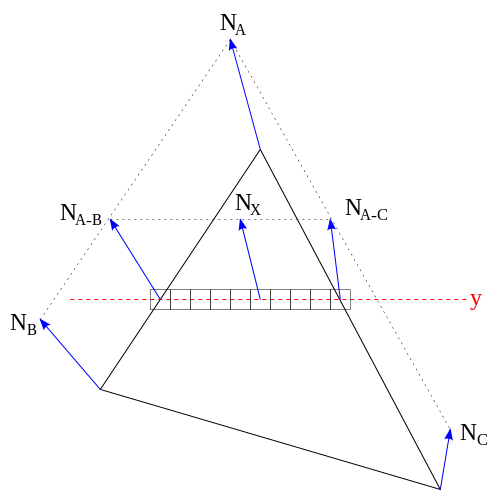
\includegraphics{pics/phongInterpol.png}
\label{fig:phongInterpo}
\caption{Normal interpolation in Phong shading}
\end{figure}
